

\documentclass{cv}

\geometry{left=6.0cm,top=1.2cm,right=1.5cm,bottom=0.7cm,nohead,nofoot}


\def\firstname{Benjamin}
\def\familyname{Vial}
\def\FileSubject{curriculum vitae}
\def\FileAuthor{\firstname~\familyname}
\def\FileTitle{\firstname~\familyname's~\FileSubject}
\def\FileKeyWords{\firstname~\familyname, \FileSubject}


\RequirePackage[unicode]{hyperref}% unicode is required for unicode pdf metadata
\hypersetup{
	breaklinks,
	baseurl       = http://,
	pdfborder     = 0 0 0,
	pdfpagemode   = UseNone,% do not show thumbnails or bookmarks on opening
	pdfstartpage  = 1,
	bookmarksopen = true,
	bookmarksdepth= 2,% to show sections and subsections
	pdfauthor   = {\FileAuthor},%
	pdftitle    = {\FileTitle},%
	pdfsubject  = {\FileSubject},%
	pdfkeywords = {\FileKeyWords},%
	pdfcreator  = {\LaTeX},
}

\addbibresource{publis.bib} % Specify the bibliography file to include publications

\begin{document}

\header{Benjamin}{~Vial}{Docteur Ingénieur | Optique, Photonique et micro-ondes}

%----------------------------------------------------------------------------------------
%	SIDEBAR SECTION
%----------------------------------------------------------------------------------------

\begin{tikzpicture}[remember picture, overlay]
	\node [anchor=north west, inner sep=0.3cm]  at (current page.north west)
	{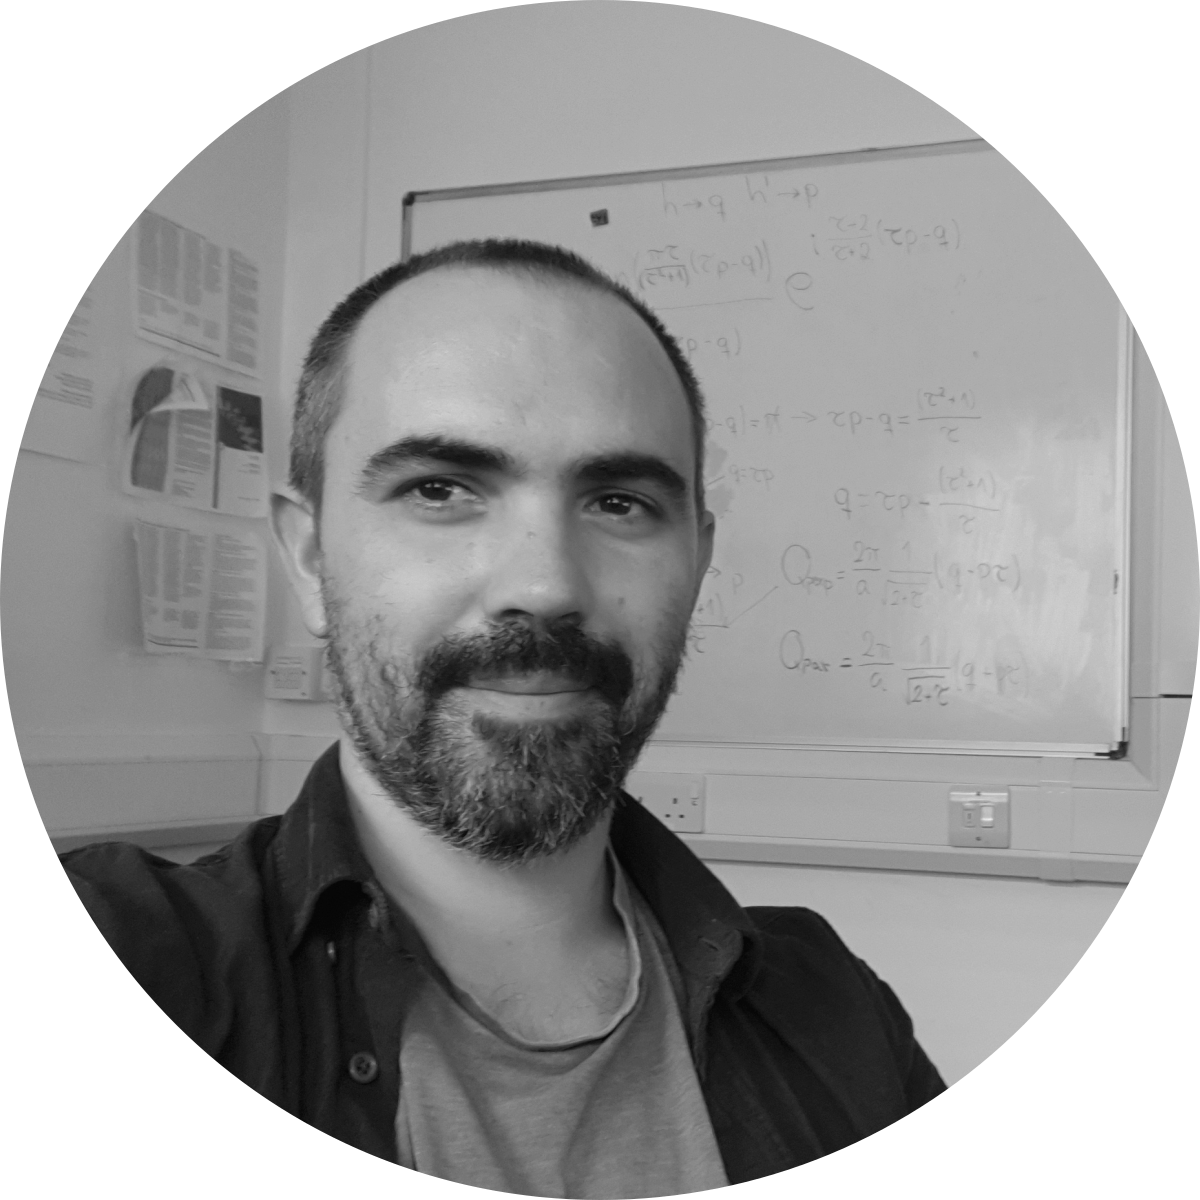
\includegraphics[height=3cm]{pic}};
\end{tikzpicture}

\begin{aside} % In the aside, each new line forces a line break
	\section{Contact}
	\faHome~~146 Glyn road
	London E5 0JE, UK
	\faPhone~~+44~7840~029~744
	\faEnvelope~~\href{mailto:b.vial@imperial.ac.uk}{b.vial@imperial.ac.uk}
	\faUser~~\href{http://bvial.info/}{bvial.info}
	\section{Informations}
	né le 09/11/1984
	nationalité française
	\section{Langues}
	français : langue maternelle
	anglais : courant
	espagnol : bases
	\section{Programmation}
	\textbf{systèmes d'exploitation}
	Linux, Windows
	\textbf{languages et scripts}
	Python, Matlab, Mathematica, \LaTeX, C, C++, Q\#, HTML, CSS
	\textbf{applications}
	git, Fenics, Gmsh, GetDP, Comsol Multiphysics, Gimp, LibreOffice, Labview
	\section{Intérêts}
	\textbf{professionels}
	Photonique
	Optique
	ingénierie micro-ondes
	processus résonants
	interaction lumière matière
	analyse modale
	domaine THz
	métamatériaux et métasurfaces
	Optique de Transformation
	modélisation numérique
	méthode des éléments finis
	méthode modale de Fourier
	FDTD
	techniques d'optimisation
	problèmes inverse
	apprentissage machine
	physique des ondes
	fabrication
	caractérisation
	science ouverte
	\textbf{personnels}
	jouer de la guitare, musique
	football, marche à pied
	voyages, cuisine
\end{aside}


%----------------------------------------------------------------------------------------
%	EDUCATION SECTION
%----------------------------------------------------------------------------------------


% \vspace*{-0.6cm}

\section{Résumé}
De formation d'ingénieur Centralien, j'ai une expertise au niveau international dans la recherche sur le contrôle des ondes par des matériaux structurés, grâce à la modélisation rigoureuse de la propagation en milieux complexes, l'optimisation et l'interface avec les expériences.

\section{Formation}

\begin{entrylist}
	%------------------------------------------------
	\entry
	{Apr. 2013}
	{Thèse de doctorat {\normalfont en Physique}}
	{\href{http://www.fresnel.fr/spip/}{Institut Fresnel}, CNRS, Centrale Marseille, Aix Marseille Universit\'e, Marseille, France}
	{Optique, Photonique et traitement d'image}
	%------------------------------------------------
	\entry
	{Oct. 2009}
	{Master {\normalfont en Physique}}
	{\href{http://www.centrale-marseille.fr/}{Centrale Marseille}~--~
		\href{http://www.lma.cnrs-mrs.fr/}{Laboratoire de Mécanique et d'Acoustique}, CNRS, Marseille, France}
	{Mécanique, Physique et Ingénierie, spécialisation en Acoustique}

	\entry
	{Oct. 2009}
	{Diplôme d'{Ingénieur Généraliste}}
	{\href{http://www.centrale-marseille.fr/}{Centrale Marseille}, Marseille, France}
	{Formation scientifique généraliste}
	%------------------------------------------------
\end{entrylist}


%----------------------------------------------------------------------------------------
%	WORK EXPERIENCE SECTION
%----------------------------------------------------------------------------------------
\vspace*{-0.2cm}
\section{Activités de recherche}

\begin{entrylist}
	\entry
	{Depuis Août 2022}
	{Postdoctorat}
	{\href{http://imperial.ac.uk/}{Imperial College London}, Londres, Royaume-Uni}
	{\href{https://www.metaveh.com/}{Projet METAVEH}: récupération d'énergie avec des métamatériaux mécaniques. Développement et optimisation de modèles de réseaux élastiques discrets et de résonateurs sur plaques minces.
	}
	%------------------------------------------------
	\entry
	{Jan. 2019 \\Juil. 2022}
	{Postdoctorat}
	{\href{http://antennas.eecs.qmul.ac.uk/}{Queen Mary, University of London}, London, UK}
	{\href{https://animate-research.com/}{Projet ANIMATE}: couplage non-linéaire et propriétés effectives de métamatériaux ferroélectriques, conception inverse pour maximiser leur ajustabilité,
		caractérisation de matériaux dans les domaines micro-ondes et THz.
	}


	\entry
	{Jan. 2017 \\Déc. 2018}
	{Postdoctorat}
	{\href{http://antennas.eecs.qmul.ac.uk/}{Queen Mary, University of London}, London, UK}
	{Projet AOTOMAT: Outils d'optimisation pour la conception de matériaux et composants électromagnétiques.
	}

	\entry
	{Juil. 2014 \\Déc. 2016}
	{Postdoctorat}
	{\href{http://antennas.eecs.qmul.ac.uk/}{Queen Mary, University of London}, London, UK}
	{\href{http://www.quest-spatial-transformation.org/}{Projet QUEST: Quest for Ultimate Electromagnetics Using Spatial Transformations.}
		Optique de Transformation appliquée à la conception, l'analyse et la caractérisation de composants à base de métamatériaux.
	}


	\entry
	{Nov. 2013\\ Jan. 2014}
	{Postdoctorat}
	{\href{http://www.fresnel.fr/}{Institut Fresnel}, Marseille, France}
	{
		Antennes résonantes. \'Etude numérique du couplage entre lumière et particules sub longueur d'onde.
		Analyse modale des résonances électriques et magnétiques pour contrôler l'émission et la densité locale d'états.
	}
	%------------------------------------------------
	\entry
	{May 2013 \\Oct. 2013}
	{Postdoctorat}
	{\href{http://www.fresnel.fr/}{Institut Fresnel}, Marseille, France}
	{
		Développement d'outils de simulation pour le tracé de rayons en milieu complexe.
	}

	%------------------------------------------------
	\entry
	{Oct. 2009\\Avr. 2013}
	{Thèse de Doctorat en Physique}
	{\href{http://www.fresnel.fr/}{Institut Fresnel}~--~\href{http://www.silios.com/}{Silios Technologies}, Marseille, France}
	{\emph{\href{http://tel.archives-ouvertes.fr/index.php?halsid=slas337fv1oqlj1okgkq7q42i5&view_this_doc=tel-00918651&version=1}
			{\'Etude de résonateurs électromagnétiques ouverts par approche modale.
				Application au filtrage multispectral dans l'infrarouge.}} (\emph{mi-temps université/entreprise})\\
		Modèles numérique part éléments finis pour le calcul des modes propres de
		l'opérateur de Maxwell pour des structures ouvertes et décomposition modale sur modes quasi-normaux.
		Application à la conception, fabrication et caractérisation de
		filtres diffractifs dans l'infrarouge pour des imageurs multispectraux: passe bande en
		transmission et coupe bande en réflexion basés sur des métamatériaux.
	}

\end{entrylist}

%----------------------------------------------------------------------------------------
%	Teaching/supervising experience SECTION
%----------------------------------------------------------------------------------------


% \vspace*{-0.2cm}
% \section{Expérience d'enseignement/encadrement}

% \begin{entrylist}
% 	%------------------------------------------------
% 	\entry
% 	{2011-2012}
% 	{Tuteur de stage}
% 	{{Institut Fresnel}, CNRS, Centrale Marseille, Marseille, France}
% 	{Optimisation de filtres spectraux diffractifs (1 élève ingénieur, 6 mois).\\
% 		Optimisation de l'absorption dans des cellules solaires (4 élèves ingénieur, 3 mois).
% 	}

% 	%------------------------------------------------
% 	\entry
% 	{2019}
% 	{Assistant d'Enseignement}
% 	{\href{http://antennas.eecs.qmul.ac.uk/}{Queen Mary, University of London}, London, UK}
% 	{Informatique quantique. Cours sur les portes et circuits quantiques. 
% 	TDs sur ordinateur et projets de fin d'année et language de programmation Q\# et Python (10 élèves de Master, 6 mois).}

% 	%------------------------------------------------

% \end{entrylist}

\vspace*{-0.2cm}
\section{Prix et récompenses}

 {Prix de la meilleure thèse 2014} {\href{https://ecole-doctorale-352.univ-amu.fr/en}{\'Ecole Doctorale 352, Physique et Science de la Matière}}

 {Prix de la meilleure thèse 2014 {\href{https://www.cnano-paca.fr/index.php?option=com_content&view=article&id=80}{CNano PACA}}, catégorie recherche finalisée}


\newgeometry{left=1.5cm,top=1.8cm,right=1.5cm,bottom=0.7cm,nohead,nofoot}



\newpage

\section{Activités pédagogiques et d'encadrement}

\begin{entrylist}

	\entry
	{fév. 2023 - sept. 2023}
	{Suivi en co-encadrement de projet de thèse}
	{Imperial College London, Londres, Royaume-Uni.}
	{Travail avec un étudiant en échange de Politechnico di Milano.\\
		\emph{Cavités isospectrales et homogénéisation en coordonnées curvilignes.}}
	\entry
	{juil. 2023 - sept. 2023}
	{Encadrement de projet de master}
	{Imperial College London, Londres, Royaume-Uni.}
	{Travail avec un étudiant du département de mathématiques].\\
		\emph{Optimisation de la dispersion pour des réseaux phononiques discrets.}}

	\entry
	{sept. 2018 - avr. 2022}
	{Suivi en co-encadrement de projets de thèse}
	{Queen Mary University of London, Londres, Royaume-Uni.}
	{Travail avec deux étudiants de thèse.\\
		\emph{Optimisation intelligente de métasurfaces avec modèles réduits.}}

	\entry
	{nov. 2019 - avr. 2020}
	{Assistant d'enseignement}
	{Queen Mary University of London, Londres, Royaume-Uni.}
	{Cours et travaux dirigés sur ordinateur pour 10 étudiants niveau Master 1.\\
		\emph{Physique et calculs quantiques, programmation en Python.}}


	\entry
	{nov. 2018 - avr. 2019}
	{Suivi en co-encadrement de projets d'élèves niveau licence}
	{Queen Mary University of London, Londres, Royaume-Uni.}
	{Encadrement d'un projet transverse et multidisciplinaire d'un groupe de quatre étudiants.\\
		\emph{Détection et reconnaissance d'émotions par mesures micro-ondes et physiologiques.}}
	\entry
	{mai-juin 2012}
	{Encadrement de stage}
	{Institut Fresnel, Marseille, France.}
	{Tuteur de stage pour un étudiant de 3ᵉ année de l'École Centrale Marseille.\\
		\emph{Optimisation de filtres multispectraux en réflexion et en transmission
			pour des applications d'imagerie infrarouge.}}



	\entry
	{jan.-fév. 2011}
	{Encadrement de projet}
	{Institut Fresnel, Marseille, France.}
	{Encadrant de projet pour cinq élèves de 2ᵉ année de l'École Centrale Marseille.\\
		\emph{Développement de cellules solaire à haut rendement à base de
			matériaux nanostructurés.}}

\end{entrylist}


\section{Activités administratives}

\begin{entrylist}

	\entry
	{nov. 2023}
	{Organisation d'une conférence}
	{Imperial College London, Londres, Royaume-Uni.}
	{Réunion et workshop sur deux projets européens. Invitations, logistique, repas, rédaction du programme.}

	\entry
	{2017}
	{Organisation de séminaires}
	{Queen Mary University of London, Londres, Royaume-Uni.}
	{
		Séminaire interne du groupe Antennas and Electromagnetics}

	\entry
	{2017-2018}
	{Rédaction de projet}
	{Queen Mary University of London, Londres, Royaume-Uni.}
	{
		Rédaction de deux projets de recherche soumis pour obtenir des financements
		de l'Engineering and Physical Sciences Research Council (EPSRC). Les deux projets (AOTOMAT et ANIMATE) ont été
		financés.}

	\entry
	{Sept. 2018- Juil. 2022}
	{Gestion de projet}
	{Queen Mary University of London, Londres, Royaume-Uni.}
	{
		Management du projet ANIMATE: création d'un espace web, organisation de réunions,
		liaison avec les partenaires industriels et académiques}


\end{entrylist}


%----------------------------------------------------------------------------------------
%	Referees contact SECTION
%----------------------------------------------------------------------------------------


% \section{Références}

% \begin{minipage}{.6\textwidth}
% 	\textbf{Prof Yang Hao}\\
% 	\faHome~~School of Electronic Engineering and Computer Science\\
% 	Queen Mary University of London\\
% 	Peter Landin Building, 10 Godward Square, Mile End Road\\
% 	London E1 4FZ, United Kingdom\\
% 	\faEnvelope~~\href{mailto:y.hao@qmul.ac.uk}{y.hao@qmul.ac.uk}\\
% 	\faPhone~~+44 20 7882 5341\\
% 	\faUser~~\href{http://www.eecs.qmul.ac.uk/~yang/}{www.eecs.qmul.ac.uk/~yang/}
% \end{minipage}%
% \begin{minipage}{0.4\textwidth}
% 	\textbf{Prof Andr\'e Nicolet}\\
% 	\faHome~~Aix-Marseille Université\\
% 	Institut Fresnel (UMR CNRS 6133)\\
% 	Domaine Universitaire de Saint-Jérôme\\
% 	F13397 Marseille cedex 20, France\\
% 	\faEnvelope~~\href{mailto:andre.nicolet@fresnel.fr}{andre.nicolet@fresnel.fr}\\
% 	\faPhone~~+33 4 91 28 87 73\\
% 	\faUser~~\href{https://www.fresnel.fr/perso/nicolet/}{www.fresnel.fr/perso/nicolet/}
% \end{minipage}


\vspace*{0.5cm}

%----------------------------------------------------------------------------------------
%	Publications SECTION
%----------------------------------------------------------------------------------------
\section{Publications et Communications\label{publis}}

\nocite{*}

\newrefcontext[labelprefix=A]
\printbibliography[type=article, title={Articles dans des revues internationales à comité de lecture}, keyword={ricl}, heading=subbibliography]

\newrefcontext[labelprefix=B]
\printbibliography[type=book, title={Contribution à un chapitre de livre}, keyword={book}, heading=subbibliography]

\newrefcontext[labelprefix=C]
\printbibliography[type=inproceedings, title={Conférences internationales avec actes}, keyword={lecture comittee}, heading=subbibliography]

\newrefcontext[labelprefix=D]
\printbibliography[type=inproceedings, title={Conférences internationales sans actes}, keyword={conference}, heading=subbibliography]

\newrefcontext[labelprefix=E]
\printbibliography[type=inproceedings, title={Conférences nationales et séminaires}, keyword={france}, heading=subbibliography]
\newrefcontext[labelprefix=F]
\printbibliography[type=thesis, title={Thèse de doctorat}, keyword={these}, heading=subbibliography]
\newrefcontext[labelprefix=G]
\printbibliography[type=article, title={En préparation}, keyword={prep}, heading=subbibliography]
\newrefcontext[labelprefix=H]
\printbibliography[type=software, title={Codes et logiciels libres}, keyword={code}, heading=subbibliography]

\end{document}
